\chapter{Schematic design}
\label{ch:schematic}

The power stage is two sheets of a KiCad 10.0.6 project that was frozen on
11 October 2026, together with the board, as revision 1.2: a sheet with the
DC-link and the terminals, and a half-bridge leg instantiated three times.
The module has 30 parts and talks to the rest of the project through 23
labelled signals (\cref{tab:interface}). This chapter explains how it is
organised and what was decided while drawing it; the two sheets close the
chapter.

\section{Sheet hierarchy}

The schematic is organised by \emph{voltage domain} rather than by function
or by phase. The three legs are one sheet drawn once and instantiated three
times: 21 of the 30 parts of the module sit on that sheet and were drawn a
single time.

\begin{table}[htbp]
\centering
\caption{Sheet hierarchy. Parts are counted per instance.}
\label{tab:sheets}
\small
\begin{tabularx}{\textwidth}{llrrY}
\toprule
Sheet & Domain & Inst. & Parts & Content \\
\midrule
root & --- & 1 & 0 & blocks, the signals between them, the requirements on the system \\
\texttt{1\_power\_stage} & HV & 1 & 9 & film DC-link capacitors, bus and phase terminals \\
\quad\texttt{leg} & HV & 3 & 7 & two \device{}, four commutation ceramics, Kelvin shunt \\
\bottomrule
\end{tabularx}
\end{table}

The sheets of gate drive, sensing, auxiliary supply, control and DC-link
management belong to the rest of the board and are outside this module.

\begin{table}[htbp]
\centering
\caption{Interface of the power-stage module: the 23 signals that leave its
sheet.}
\label{tab:interface}
\small
\begin{tabularx}{\textwidth}{lYrl}
\toprule
Group & Signals & Count & Goes to \\
\midrule
DC-link & \texttt{HV\_DCP}, \texttt{HV\_DCN} & 2 & gate drive, DC-link management \\
Switching nodes & \texttt{HV\_SW1}, \texttt{HV\_SW2}, \texttt{HV\_SW3} & 3 & gate drive \\
Gate and Kelvin source & \texttt{GHk\_GATE}, \texttt{GHk\_COM}, \texttt{GLk\_GATE}, \texttt{GLk\_COM}, $k = 1,2,3$ & 12 & gate drive \\
Shunt voltage & \texttt{SNSk\_SP}, \texttt{SNSk\_SN}, $k = 1,2,3$ & 6 & phase-current sensing \\
\bottomrule
\end{tabularx}
\end{table}

\section{Net naming and net classes}

Net names carry their voltage domain as a prefix, so that whether a net is
hazardous can be read from its name and enforced by a net class. The
floating gate references of the six devices are deliberately distinct names
rather than a shared one: they move by hundreds of volts with respect to one
another during commutation, and merging them would be an error that ERC
cannot detect.

The net classes follow the same rule: one class per domain. A first version
had a single class for all gate domains and asked for
\SI{4.5}{\milli\metre} between any two of its nets. That is wrong inside a
domain: the gate and the Kelvin source of one device are the same domain and
sit \SI{0.70}{\milli\metre} apart on the package. With one class per domain
the clearance \emph{inside} a class is the manufacturing value, and the
distances \emph{between} classes are set by the rules of the board.

\begin{table}[htbp]
\centering
\caption{Net classes of the power stage. Clearance and track width are the
values inside the class; between classes the rules of the board apply.}
\label{tab:netclasses}
\small
\begin{tabularx}{\textwidth}{lYrr}
\toprule
Class & Nets & Clearance & Track \\
\midrule
\texttt{HV\_BUS}   & DC-link positive and negative & \SI{2.0}{\milli\metre} & \SI{10.4}{\milli\metre} \\
\texttt{HV\_POWER} & switching nodes and phase outputs & \SI{2.0}{\milli\metre} & \SI{8.4}{\milli\metre} \\
\texttt{GATE\_H1} \ldots\ \texttt{GATE\_DIS} & floating gate domains, one class each & \SI{0.3}{\milli\metre} & \SI{0.5}{\milli\metre} \\
\bottomrule
\end{tabularx}
\end{table}

\section{Reference designators}

References encode position in the hierarchy: the hundreds give the sheet, the
tens the instance, the units the part within it. The high-side device of
leg~2 is \texttt{Q121}, the driver of the high side of leg~1 is
\texttt{U211}, the amplifier of phase~1 is \texttt{U321}, the bus amplifier
\texttt{U601}. A reference read on the board therefore says where to look in
the schematic, and the same part has the same last digit in every instance.

\section{Components of the power stage}

\Cref{tab:components} lists every part of the module with the reason it was
chosen. Giving each part a unique order code meant opening its datasheet, and
for the commutation ceramics the datasheet contradicted an assumption of the
preceding chapters: in C0G at \SI{1200}{\volt} the largest ceramic is
\SI{47}{\nano\farad} in a 3640~\cite{kemet_kclink}, and the \SI{220}{\nano\farad}
of the earlier estimate does not exist in that class.

\begin{table}[htbp]
\centering
\caption{Components of the power stage, with the basis of each choice.}
\label{tab:components}
\label{tab:captdecisions}
\small
\begin{tabularx}{\textwidth}{L{0.16\textwidth}L{0.2\textwidth}L{0.15\textwidth}Y}
\toprule
Function (quantity) & Part & Key values & Chosen because \\
\midrule
Switching devices (6) & E3M0016120K, Wolfspeed~\cite{wolfspeed_e3m0016}
  & \SI{1200}{\volt}, \SI{16}{\milli\ohm}, TO-247-4L
  & passes C1--C4 with the vendor SPICE model (\cref{sec:deviceselection}) \\
DC-link film (2) & MKP1848 \SI{140}{} and \SI{60}{\micro\farad}, Vishay~\cite{vishay_mkp1848}
  & \SI{200}{\micro\farad}, \SI{1100}{\volt} DC
  & ripple \SI{2.86}{\volt} in the worst case against \SI{4}{\volt}; the \SI{1100}{\volt} class carries \SI{900}{\volt} up to a \SI{98}{\celsius} hotspot (\cref{sec:dclink}) \\
Commutation ceramics (12, four per leg) & CKC33C473\-KEGACAUTO, KEMET~\cite{kemet_kclink}
  & \SI{47}{\nano\farad} C0G, \SI{1200}{\volt}, 3640
  & \SI{188}{\nano\farad} per leg at \SI{75}{\percent} of the rating at \SI{900}{\volt}; \SI{6.25}{\milli\metre} between pads against \SI{2.80}{\milli\metre} of creepage; no bias loss \\
Phase shunts (3) & CSS2H-3920R-L500FE, Bourns
  & \SI{0.5}{\milli\ohm}, Kelvin
  & \SI{0.45}{\watt} at rated current, \SI{0.90}{\watt} stalled, terminals at most \SI{115}{\celsius} (\cref{sec:complife}) \\
Insulating pad (one per leg) & aluminium nitride \SI{0.63}{\milli\metre} with phase-change interface
  & $\Rthcs \leq \SI{0.18}{\celsius\per\watt}$
  & the interfaces, not the ceramic, set the value (\cref{sec:coolalt}) \\
Cooling rail (1) & six-port aluminium extrusion, \SI{10}{\litre\per\minute}
  & $R_\mathrm{eq} = \SI{0.069}{\celsius\per\watt}$
  & the rail as first drawn, with two channels, reaches \SI{128.7}{\celsius} at locked rotor, beyond C1 (\cref{sec:cooling}) \\
\bottomrule
\end{tabularx}
\end{table}

\section{Footprint of the power device}

\begin{finding}{The package pitch is not the one initially assumed}
The TO-247-4L pad spacing is \emph{not} the uniform \SI{5.45}{\milli\metre}
of the three-lead TO-247. From the recommended pad layout of the device
datasheet~\cite{wolfspeed_e3m0016} it is \SI{5.08}{\milli\metre} between pins 1
and 2 and \SI{2.54}{\milli\metre} between the remaining pins, for a total
span of \SI{10.16}{\milli\metre}.

The consequence for insulation coordination is larger than a change of
pitch, because the pitch is not the creepage. Pins 1 and 2 are the
drain--source pair, and with pads \SI{1.84}{\milli\metre} wide on a
\SI{5.08}{\milli\metre} pitch the copper-to-copper gap is
\SI{3.24}{\milli\metre}: that, and not \SI{5.45}{\milli\metre}, is the
worst-case creepage between high-voltage nodes on the board. The gate is
\SI{10.16}{\milli\metre} from the drain and is not the critical pair.

\SI{3.24}{\milli\metre} is \SI{2.8}{} times less than the
\SI{9.00}{\milli\metre} that IEC 60664-1~\cite{iec60664} asks for at the
\SI{900}{\volt} working voltage in pollution degree 2 on ordinary FR-4, and
the package leaves no room to do better. Conformal coating brings the
pollution degree to 1, where the requirement is \SI{2.80}{\milli\metre} and
the same \SI{3.24}{\milli\metre} passes with \SI{16}{\percent} of margin. The full
coordination, including the reinforced barrier and the two paths that this
first pass missed, is in \cref{sec:insulation}.

The lesson concerns method: a constraint that
the package imposes on the \emph{process} was found by measuring the
footprint, and would not have been found by reading the pitch.
\end{finding}

\section{Schematic sheets}

The two sheets of the module follow, one per page, in the order of
\cref{tab:sheets}. Of the leg sheet one instance is shown, leg~1; the others
differ only in their references.

\newcommand{\foglio}[3]{%
  \begin{sidewaysfigure}
    \centering
    \includegraphics[page=#1,width=\textwidth,height=0.86\textheight,keepaspectratio]{figures/kicad_schema.pdf}
    \caption{#2}
    \label{fig:sch-#3}
  \end{sidewaysfigure}}

\foglio{2}{Power stage: DC-link film capacitors, terminals and the three legs.}{power}
\foglio{3}{Half-bridge leg (leg 1 of 3): devices, commutation ceramics, Kelvin shunt.}{leg}
